\documentclass[letterpaper]{article}
\usepackage[margin=1.0in]{geometry}
% -----PACKAGES
%\usepackage[shortend,titlenumbered]{algorithm2e}
%\usepackage{algorithmic}
%\usepackage[plain]{algorithm}
\usepackage{multicol}
\usepackage{color}
\usepackage{multirow}
\usepackage{fancybox}
%\usepackage{index}
\usepackage{varioref}
\usepackage{psfrag}
\usepackage{epsfig}
\usepackage{boxedminipage}
\usepackage{graphicx}
\usepackage{rotating}
\usepackage{amsmath}
\usepackage{amssymb}
%\usepackage{amsfont}
\usepackage{latexsym}
\usepackage{alltt}
%\usepackage[small,bf]{caption}
\usepackage{url}
%\usepackage{citesort}
%\usepackage{crop}
\usepackage{array}
\usepackage{subfigure}
\usepackage{dcolumn}

% -----SETLENGTH
%\setlength{\captionmargin}{20pt} 

% -----NEWCOMMANDS
\newcommand{\nc}{\newcommand}
\nc{\mathsm}[1]{\text{\small{$#1$}}}
\nc{\ubar}[1]{\underset{-}{#1}}
\nc{\optype}{\textrm}
\nc{\EQ}[1]{(\ref{eq:#1})}
\nc{\TAB}[1]{\ref{tab:#1}}
\nc{\FIG}[1]{\ref{fig:#1}}
\nc{\SEC}[1]{\ref{sec:#1}}
\nc{\ALG}[1]{\ref{alg:#1}}
\nc{\CHAP}[1]{\ref{chap:#1}}
\nc{\mtrx}[1]{\boldsymbol{\mathbf{#1}}}
\nc{\vctr}[1]{\boldsymbol{\mathbf{#1}}}
\nc{\grad}{\mbox{\boldmath$\nabla$}}
\nc{\gradient}{\textsl{grad}\,}
\nc{\hessian}{\textsl{grad\,}^2}
\nc{\ii}{\iota}
\nc{\dd}{d}
\nc{\ee}{\mathrm{e}}
\nc{\pdiv}[2]{\partial{#1}/\partial{#2}}
\nc{\dpdiv}[2]{\displaystyle{\frac{\partial{#1}}{\partial{#2}}}}
\nc{\ddiv}[2]{\displaystyle{\frac{\dd{#1}}{\dd{#2}}}}
\nc{\inpr}{\hspace{-1pt}\cdot\hspace{-1pt}}
\nc{\IR}{\mathbb{R}}
\nc{\IN}{\mathbb{N}}
\nc{\IZ}{\mathbb{Z}}
\nc{\IC}{\mathbb{C}}
\nc{\half}{\frac{1}{2}}
\nc{\shalf}{\scriptstyle{\half}} 
\nc{\ds}[1]{\displaystyle{#1}}
\nc{\ts}[1]{\textstyle{#1}}
\nc{\sign}{\optype{sign}}
\nc{\spr}{\optype{spr}}
\nc{\dist}{\optype{dist}}
\nc{\rank}{\optype{rank}}
\nc{\codim}{\optype{codim}}
\nc{\supp}{\optype{supp}}
\nc{\diag}{\optype{diag}}
\nc{\meas}{\optype{meas}}
\nc{\cond}{\optype{cond}}
\nc{\kernel}{\optype{kernel}}
\nc{\spa}{\optype{span}}
\nc{\order}{\mathcal{O}}
\nc{\Fr}{\mathrm{Fr}}
\nc{\Rey}{\mathrm{Re}}
\nc{\Ord}{O}
\nc{\ord}{o}
\nc{\st}{\:{:}\:}
\nc{\closure}[1]{\overline{#1}}
\nc{\emin}[1]{\emph{#1}\index{#1}\/}
\nc{\rmin}[1]{#1\index{{}@{#1}}}
\nc{\Laplace}{\Delta}
\nc{\ie}{i.e.}
\nc{\eg}{e.g.}
%\nc{\union}{\cup}
\nc{\Union}{\bigcup}
\nc{\lf}[1]{\mathsf{#1}}
\nc{\dbar}[1]{\bar{\bar{#1}}}
\nc{\ul}[1]{\underline{#1}}
\nc{\hpt}{\hspace{0.5pt}}
\nc{\E}[1]{\times{}10^{#1}}
\nc{\inp}[2]{\langle{#1},{#2}\rangle}
\nc{\tmpcommand}{}

% -----RENEWCOMMANDS
\renewcommand{\baselinestretch}{1}
\renewcommand{\exp}{\optype{exp}\,}
\renewcommand{\cosh}{\optype{cosh}\,}
\renewcommand{\tanh}{\optype{tanh}\,}
\renewcommand{\sinh}{\optype{sinh}\,}
\renewcommand{\div}[1]{\optype{div}\,{#1}}
\renewcommand{\half}{\mbox{$\frac{1}{2}$}}
%\renewcommand{\descriptionlabel}[1]{\hspace{\labelsep}\emph{#1}}

% -----ETC
\raggedbottom


\DeclareMathOperator{\curl}{\bf curl}
\DeclareMathOperator{\rot}{\rm curl}
\DeclareMathOperator{\divv}{\rm div}
\newcommand{\tro}{\gamma_0}
\newcommand{\trt}{\gamma_{\sft}}
\newcommand{\trn}{\gamma_{\sfn}}

\newcommand{\PT}{{\partial T}}
\newcommand{\bbN}{{\mathbb{N}}}
\newcommand{\bbP}{{\mathbb{P}}}

\newcommand{\scC}{{\mathscr{C}}}
\newcommand{\caD}{{\mathcal{D}}}
\newcommand{\caL}{{\mathcal{L}}}

\newcommand{\sfe}{{\mathsf{e}}}
\newcommand{\sff}{{\mathsf{f}}}
\newcommand{\sft}{{\boldsymbol{\mathsf{t}}}}
\newcommand{\sfn}{{\boldsymbol{\mathsf{n}}}}

%   Common caligraphic abbrevs
\newcommand{\BB}{\mathcal{B}}
\newcommand{\CC}{\mathcal{C}}
\newcommand{\DD}{\mathcal{D}}
\newcommand{\EE}{\mathcal{E}}
\newcommand{\FF}{\mathcal{F}}
\newcommand{\GG}{\mathcal{G}}
\newcommand{\II}{\mathcal{I}}
\newcommand{\JJ}{\mathcal{J}}
\newcommand{\KK}{\mathcal{K}}
\newcommand{\LL}{\mathcal{L}}
\newcommand{\OO}{\mathcal{O}}
\newcommand{\QQ}{\mathcal{Q}}
\newcommand{\RR}{\mathcal{R}}
\newcommand{\TT}{\mathcal{T}}


 %% JAY'S PREAMBLE
 %%========================

%   Math symbol definitions
\def\d{\partial}
%\newsymbol\lee 132E
\newcommand{\union}{\mathop{\bigcup}}
\newcommand{\intersect}{\mathop{\bigcap}}
\newcommand{\binomial}[2]{\ensuremath{
		\begin{pmatrix}{#1}\\{#2}\end{pmatrix}}}
\newcommand{\smallbinomial}[2]{\ensuremath{
		(\begin{smallmatrix}{#1}\\{#2}\end{smallmatrix})}}
\newcommand{\tang}[1]{\ensuremath{{#1}_{\intercal}}} % can use \top
						     % also
\newcommand{\hypergeom}[2]{\ensuremath{\sideset{_{#1}}{_{#2}}{\mathop{F}}}}
%   Difficult names
\newcommand{\Babuska}{Babu{\v{s}}ka}       % Remember: Usage is \Babuska\
\newcommand{\Cea}{C{\'e}a}                 % with trailing `\' to give space
\newcommand{\Poincare}{Poincar{\'{e}}}     % when needed, but when ending
\newcommand{\Nedelec}{N{\'{e}}d{\'{e}}lec} % sentence use \Babuska.
\newcommand{\Frechet}{Fr{\'{e}}chet}
\newcommand{\Muller}{M{\"u}ller}
\newcommand{\LHospital}{L'H{\^{o}}spital}
%   Bold and beautiful
\newcommand{\ba}{{\boldsymbol{a}}}
\newcommand{\bA}{\boldsymbol{A}}
\newcommand{\balpha}{{\boldsymbol{\alpha}}}
\newcommand{\bB}{{\boldsymbol{B}}}
\newcommand{\bb}{{\boldsymbol{b}}}
\newcommand{\bbeta}{{\boldsymbol{\beta}}}
\newcommand{\etab}{{\boldsymbol{\eta}}}
\newcommand{\bC}{{\boldsymbol{C}}}
\newcommand{\bc}{{\boldsymbol{c}}}
\newcommand{\bD}{{\boldsymbol{D}}}
\newcommand{\bd}{{\boldsymbol{d}}}
\newcommand{\db}{{\boldsymbol{\d}}}
\newcommand{\bdelta}{{\boldsymbol{\delta}}}
\newcommand{\bDelta}{{\boldsymbol{\Delta}}}
\newcommand{\beps}{{\boldsymbol{\varepsilon}}}
\newcommand{\be}{{\boldsymbol{e}}}
\newcommand{\bg}{{\boldsymbol{g}}}
\newcommand{\bm}{{\boldsymbol{m}}}
\newcommand{\bn}{{\boldsymbol{n}}}
\newcommand{\bN}{{\boldsymbol{N}}}
\newcommand{\bp}{{\boldsymbol{p}}}
\newcommand{\bpsi}{{\boldsymbol{\psi}}}
\newcommand{\bq}{{\boldsymbol{q}}}
\newcommand{\bxi}{{\boldsymbol{\xi}}}
\newcommand{\bE}{{\boldsymbol{E}}}
\newcommand{\bF}{{\boldsymbol{F}}}
\newcommand{\bh}{{\boldsymbol{h}}}
\newcommand{\bH}{{\boldsymbol{H}}}
\newcommand{\bI}{{\boldsymbol{I}}}
\newcommand{\bj}{{\boldsymbol{j}}}
\newcommand{\bJ}{{\boldsymbol{J}}}
\newcommand{\bK}{{\boldsymbol{K}}}
\newcommand{\bk}{{\boldsymbol{k}}}
\newcommand{\bll}{{\boldsymbol{\ell}}}
\newcommand{\bL}{{\boldsymbol{L}}}
\newcommand{\blambda}{{\boldsymbol{\lambda}}}
\newcommand{\bmu}{{\boldsymbol{\mu}}}
\newcommand{\bM}{{\boldsymbol{M}}}
\newcommand{\bomega}{{\boldsymbol{\omega}}}
\newcommand{\bP}{{\boldsymbol{P}}}
\newcommand{\bphi}{{\boldsymbol{\phi}}}
\newcommand{\bQ}{{\boldsymbol{Q}}}
\newcommand{\bG}{{\boldsymbol{G}}}
\newcommand{\bu}{{\boldsymbol{u}}}
\newcommand{\bU}{{\boldsymbol{U}}}
\newcommand{\bV}{{\boldsymbol{V}}}
\newcommand{\bX}{{\boldsymbol{X}}}
\newcommand{\bv}{{\boldsymbol{v}}}
\newcommand{\bw}{{\boldsymbol{w}}}
\newcommand{\bW}{{\boldsymbol{W}}}
\newcommand{\bR}{{\boldsymbol{R}}}
\newcommand{\br}{{\boldsymbol{r}}}
\newcommand{\bS}{{\boldsymbol{S}}}
\newcommand{\bT}{{\boldsymbol{T}}}
\newcommand{\btau}{{\boldsymbol{\tau}}}
\newcommand{\bt}{{\boldsymbol{t}}}
\newcommand{\bx}{{\boldsymbol{x}}}
\newcommand{\by}{{\boldsymbol{y}}}
\newcommand{\bz}{{\boldsymbol{z}}}
\newcommand{\bzero}{{\boldsymbol{0}}}
\newcommand{\bZ}{{\boldsymbol{Z}}}
%   Common scalar fields
\newcommand{\RRR}{\mathbb{R}}
\newcommand{\CCC}{\mathbb{C}}
\newcommand{\ZZZ}{\mathbb{Z}}
\newcommand{\NNN}{\mathbb{N}}
%   Differential operators
\newcommand{\dive}{\mathop\mathrm{div}}
%\newcommand{\grad}{\ensuremath{\mathop{{\bf{grad}}}}}
%\newcommand{\curl}{{\ensuremath\mathop{\mathbf{curl}\,}}}
\newcommand{\Curl}{ {\bf Curl}}
\newcommand{\dx}{\ensuremath{\mathrm{d}x}}
\newcommand{\dy}{\ensuremath{\mathrm{d}y}}
\newcommand{\dr}{\ensuremath{\mathrm{d}r}}
\newcommand{\dR}{\ensuremath{\mathrm{d}R}}
\newcommand{\drho}{\ensuremath{\mathrm{d}\rho}}
\newcommand{\dz}{\ensuremath{\mathrm{d}z}}
\newcommand{\dzeta}{\ensuremath{\mathrm{d}\zeta}}
%   Wordy math symbols
\newcommand{\card}{\ensuremath{\mathop\mathrm{card}}}
%\newcommand{\diag}{\ensuremath{\mathop\mathrm{diag}}}
\newcommand{\diam}{\ensuremath{\mathop\mathrm{diam}}}
%\newcommand{\dist}{\mathop\mathrm{dist}}
\newcommand{\Ker}{\mathop\mathrm{Ker}}
\newcommand{\Range}{\mathop\mathrm{Range}}
%\newcommand{\rank}{\mathop\mathrm{rank}}
%\newcommand{\meas}{\mathop\mathrm{meas}}
\newcommand{\Forall}{\quad\text{for all }}
%\newcommand{\supp}{\mathop\mathrm{supp}}
\newcommand{\Span}{\mathop\mathrm{Span}}
\newcommand{\Hdiv}[1]{\bH(\dive,#1)}
%\newcommand{\Hcurl}[1]{\bH(\curl,#1)}
%   Common caligraphic abbrevs
%\newcommand{\BB}{\mathcal{B}}
%\newcommand{\CC}{\mathcal{C}}
%\newcommand{\DD}{\mathcal{D}}
%\newcommand{\EE}{\mathcal{E}}
%\newcommand{\FF}{\mathcal{F}}
%\newcommand{\GG}{\mathcal{G}}
%\newcommand{\II}{\mathcal{I}}
%\newcommand{\JJ}{\mathcal{J}}
%\newcommand{\KK}{\mathcal{K}}
%\newcommand{\LL}{\mathcal{L}}
%\newcommand{\OO}{\mathcal{O}}
%\newcommand{\QQ}{\mathcal{Q}}
%\newcommand{\RR}{\mathcal{R}}
%\newcommand{\TT}{\mathcal{T}}
%   Variations on standard symbols
\newcommand{\veps}{\varepsilon}
\newcommand{\vlam}{\varLambda}
\newcommand{\vpi}{\varPi}
\newcommand{\vPi}{\boldsymbol{\varPi}}
\newcommand{\vsig}{\varSigma}
\newcommand{\vbt}{\boldsymbol{\varTheta}}
\newcommand{\vPsi}{\boldsymbol{\varPsi}}
%\newcommand{\ii}{\hat{\imath}}
%   Innerproducts, norms, etc
\newcommand{\ntrip}[1]{|\!|\!| {#1} |\!|\!|}
\newcommand{\ip}[1]{\langle {#1} \rangle}
%   Utilities
\newcommand{\blnk}{\underline{\hspace{3cm}}\;}
\newcommand{\marg}[1]{\marginpar{\tiny{\framebox{\parbox{1.7cm}{#1}}}}}
\newcommand{\degreeC}[1]{\ensuremath{{#1\,}^\circ\!\text{C}}}
                        % try also  \textcelsius of textcomp package
%   Trademarked names \texttrademark, \textregistered
\newcommand{\matlab}{MATLAB\textregistered\renewcommand{\matlab}{MATLAB}}
\newcommand{\femlab}{FEMLAB\textregistered\renewcommand{\femlab}{FEMLAB}}

%   Style preferences
\renewcommand{\thefootnote}{\fnsymbol{footnote}} % Use symbols instead of
						 % numbers for footnotes
						 

\newcommand{\Eg}{\EE^\mathrm{grad}}
\newcommand{\Ec}{\boldsymbol{\EE}^\mathrm{curl}}
\newcommand{\Ed}{\boldsymbol{\EE}^\mathrm{div}}


\newcommand{\bfdu}{\mbox{\boldmath $\delta u$}}
\newcommand{\bfdv}{\mbox{\boldmath $\delta v$}}
\newcommand{\du}{{\delta u}}
\newcommand{\dv}{{\delta v}}
\newcommand{\bfnabt}{\widetilde{\bfnab}}
\newcommand{\bfepst}{\widetilde{\bfeps}}

\graphicspath{{../Proposal/figs/}}

\title{Space-Time DPG: Designing a Method for Massively Parallel CFD}
\author[1]{Truman Ellis}
\author[1]{Leszek Demkowicz}
\author[2]{Nathan Roberts}
\author[3]{Jesse Chan}
\author[1]{Robert Moser}
\affil[1]{Institute for Computational Engineering and Sciences, University of Texas at Austin}

\affil[2]{Argonne Leadership Computing Facility, Argonne National Laboratory}

\affil[3]{Computational and Applied Math, Rice University}
\date{}

\begin{document}
\maketitle

\begin{abstract}
The discontinuous Petrov-Galerkin method is a novel finite element framework with exceptional stability and adaptivity properties.
Initial mesh design is a time consuming and expensive part of CFD simulations as a domain expert has to manually design the 
mesh to achieve near resolution in all parts of the domain lest the numerical method become unstable.
DPG in contrast does not have a pre-asymptotic regime, allowing simulations to start on the coarsest mesh that can adequately represent the domain geometry.
\emph{A posteriori} error estimation and adaptivity can also be done very naturally as DPG comes with an error representation function 
that indicates error in the energy norm.

Automatic adaptivity and pre-asymptotic stability produce a powerful synergy when combined with high performance computing.
Human intervention to correct or adapt a failed massively parallel simulation can be a costly endeavor, prompting the desire for a
numerical technology that will automatically adapt to changing physical dynamics while avoiding ``crashing'' due to under-resolved meshes.
An ideal parallel algorithm should be locally compute intensive while maintaining minimal memory requirements.
These are all observed properties of the discontinuous Petrov-Galerkin finite element method.
Locally computed \emph{optimal test functions} ensure stability on convection dominated flows as well as resolved viscous flow.
Individual contributions from each element to the global stiffness matrix can be computed completely independently due to the discontinuous nature of DPG.
Furthermore, static condensation allows the global solve to concern only the \emph{trace} degrees of freedom; 
trace variables are defined on the mesh skeleton.  
This allows significant reduction of the cost of the global solve.  
The internal degrees of freedom can then be resolved using a fully parallel post-processing step.

We recently began exploring the extension of these attractive DPG properties to space-time domains, allowing us to automate and localize temporal adaptivity
in the same way that we already do with spatial adaptivity. Preliminary results have been generated with Camellia\cite{Roberts2011} for spatially 1D flows,
and a rewrite of Camellia for higher dimensions is currently in progress.
\end{abstract}

%   /$$$$$$             /$$                               /$$                       /$$     /$$                    
%  |_  $$_/            | $$                              | $$                      | $$    |__/                    
%    | $$   /$$$$$$$  /$$$$$$    /$$$$$$   /$$$$$$   /$$$$$$$ /$$   /$$  /$$$$$$$ /$$$$$$   /$$  /$$$$$$  /$$$$$$$ 
%    | $$  | $$__  $$|_  $$_/   /$$__  $$ /$$__  $$ /$$__  $$| $$  | $$ /$$_____/|_  $$_/  | $$ /$$__  $$| $$__  $$
%    | $$  | $$  \ $$  | $$    | $$  \__/| $$  \ $$| $$  | $$| $$  | $$| $$        | $$    | $$| $$  \ $$| $$  \ $$
%    | $$  | $$  | $$  | $$ /$$| $$      | $$  | $$| $$  | $$| $$  | $$| $$        | $$ /$$| $$| $$  | $$| $$  | $$
%   /$$$$$$| $$  | $$  |  $$$$/| $$      |  $$$$$$/|  $$$$$$$|  $$$$$$/|  $$$$$$$  |  $$$$/| $$|  $$$$$$/| $$  | $$
%  |______/|__/  |__/   \___/  |__/       \______/  \_______/ \______/  \_______/   \___/  |__/ \______/ |__/  |__/
%                                                                                                                  
%                                                                                                                  
% 
\section{Introduction}

%    /$$$$$$  /$$                   /$$                                     /$$    
%   /$$__  $$| $$                  | $$                                    | $$    
%  | $$  \ $$| $$$$$$$   /$$$$$$$ /$$$$$$    /$$$$$$   /$$$$$$   /$$$$$$$ /$$$$$$  
%  | $$$$$$$$| $$__  $$ /$$_____/|_  $$_/   /$$__  $$ |____  $$ /$$_____/|_  $$_/  
%  | $$__  $$| $$  \ $$|  $$$$$$   | $$    | $$  \__/  /$$$$$$$| $$        | $$    
%  | $$  | $$| $$  | $$ \____  $$  | $$ /$$| $$       /$$__  $$| $$        | $$ /$$
%  | $$  | $$| $$$$$$$/ /$$$$$$$/  |  $$$$/| $$      |  $$$$$$$|  $$$$$$$  |  $$$$/
%  |__/  |__/|_______/ |_______/    \___/  |__/       \_______/ \_______/   \___/  
%                                                                                  
%                                                                                  
%        
\section{Abstract Derivation of DPG}

\subsection{Adaptivity}

\subsection{Parallelization}

\section{Space-Time Model Problems}

%   /$$   /$$                       /$$    
%  | $$  | $$                      | $$    
%  | $$  | $$  /$$$$$$   /$$$$$$  /$$$$$$  
%  | $$$$$$$$ /$$__  $$ |____  $$|_  $$_/  
%  | $$__  $$| $$$$$$$$  /$$$$$$$  | $$    
%  | $$  | $$| $$_____/ /$$__  $$  | $$ /$$
%  | $$  | $$|  $$$$$$$|  $$$$$$$  |  $$$$/
%  |__/  |__/ \_______/ \_______/   \___/  
%                                          
%                                          
%  
The simplest space-time problem we can consider where the the spatial and temporal dimensions are treated differently is the heat equation.
We start with a general $n$-dimensional spatial derivation and later simplify to spatially 1D with a few numerical experiments.

\subsection{Derivation}
Let $\Omega(t)\subset\mathbb{R}^d$ be the spatial domain with boundary $\partial\Omega$.
The heat equation is
\begin{equation}
	\frac{\partial u}{\partial t}-\epsilon\Delta u=f\,,\quad\bfx\in\Omega\,,\;t\in(t_0,T)
\end{equation}
where $u$ is unknown heat, $\epsilon$ is the diffusion scale, $f$ is the source term, $t_0$ is the start time, and $T$ is the final time.
Let $Q\subset\mathbb{R}^{d+1}$ denote the full space-time domain which is then tessellated into space-time elements $K$.

Let us proceed as usual and form a system of first order equations:
\begin{equation}
\label{eq:heatFirstOrder}
\begin{aligned}
\bfsigma-\epsilon\Grad u&=0\\
\frac{\partial u}{\partial t}-\Div\bfsigma&=f\,.
\end{aligned}
\end{equation}
Let us say that $f\in\LQ$, then we seek $u$, and $\bfsigma$ such that $u,\,\bfsigma,\,\Grad u,\,\frac{\partial u}{\partial t}-\Div\bfsigma\in\LQ$.
Notice that this is a weaker condition than saying $\frac{\partial u}{\partial t}\in\LQ$ and $\Div\bfsigma\in\LQ$.
It helps to view $\bfU:=(-\bfsigma, u)$ as a group variable in space-time. 
Then the last condition is telling us that $\Divxt\bfU\in\LQ$, or that $\bfU\in\HdivQ$.
That is to say the normal component $-\bfsigma\cdot\bfn_x+u\cdot n_t$ (which we call the flux) is continuous across element faces, 
where $\bfn=(\bfn_x,n_t)^T$ is the full space-time normal vector for element $K$.
Now consider the condition that $\Grad u\in\LQ$.
This implies that $u$ lives in a tensor product space of $H^1$ spatially and $L^2$ temporally and that
$u\cdot n_t$ is continuous on element faces where $n_t$ is nonzero; we call this the spatial trace.

Now that we understand which Sobolev spaces $u$ and $\bfsigma$ live in, we can proceed with a derivation of the space-time DPG formulation for this problem.
We multiply the first equation in \eqref{eq:heatFirstOrder} by test function $\bftau$ and the second by $v$. Then we integrate by parts over each element:
\begin{equation}
\label{eq:heatBF}
	\begin{aligned}
		\LRp{\bfsigma,\bftau}+\epsilon\LRp{u,\Div\bftau}-\LRa{\hat u,\tau_n}&=0\\
		-\LRp{u,\frac{\partial v}{\partial t}}+\LRp{\bfsigma,\Grad v}-\LRa{\hat t,v}&=\LRp{f,v}\,,
	\end{aligned}
\end{equation}
where $\hat u$ is the spatial trace and $\hat t$ is the flux.
The second equation could alternatively be written in terms of the group variable $\bfU$:
\begin{equation}
\label{heatBFAlt}
-\LRp{\bfU,\Gradxt v}-\LRa{\hat t,v}=\LRp{f,v}\,.
\end{equation}
This alternate version emphasizes the definition of the flux: $\hat t=\trace\LRp{-\bfsigma}\cdot\bfn_x+\trace{(u)}\cdot n_t$.
From \eqref{eq:heatBF} and \eqref{heatBFAlt} it is clear that $\bftau\in\HdivK$ where the divergence is taken only over spatial directions, and $v\in\HOneK$.
Figure \ref{fig:heatMesh} illustrates the support for the fluxes and spatial traces. Notice that the fluxes live on all element boundaries, while the spatial traces only live on ``non-horizontal'' edges.

\begin{figure}[h!]
\begin{center}
\begin{tikzpicture}[line cap=round,line join=round,>=triangle 45,x=2.0cm,y=2.0cm]
\clip(-0.7,-1.01) rectangle (5.27,2.29);
\draw (0,2)-- (0,0);
\draw (0,0)-- (1,0);
\draw (1,0)-- (4,0);
\draw (4,0)-- (5,0);
\draw (5,0)-- (5,2);
\draw (5,2)-- (3,2);
\draw (3,2)-- (2,2);
\draw (2,2)-- (0,2);
\draw (1,0)-- (1.5,1);
\draw (1.5,1)-- (2,2);
\draw (1.5,1)-- (3.5,1);
\draw (3,2)-- (3.5,1);
\draw (3.5,1)-- (4,0);
\draw (-0.21,0.9) node[anchor=south west] {$\hat u$};
\draw (4.82,0.9) node[anchor=south west] {$\hat u$};
\draw (3.5,0.45) node[anchor=south west] {$\hat u$};
\draw (1.0,0.45) node[anchor=south west] {$\hat u$};
\draw (1.5,1.4) node[anchor=south west] {$\hat u$};
\draw (3.0,1.4) node[anchor=south west] {$\hat u$};
\draw (0.05,0.9) node[anchor=south west] {$\hat t$};
\draw (1.40,0.45) node[anchor=south west] {$\hat t$};
\draw (3.79,0.45) node[anchor=south west] {$\hat t$};
\draw (2.47,1.0) node[anchor=south west] {$\hat t$};
\draw (3.33,1.4) node[anchor=south west] {$\hat t$};
\draw (1.89,1.4) node[anchor=south west] {$\hat t$};
\draw (5.07,0.9) node[anchor=south west] {$\hat t$};
\draw (4.44,0.0) node[anchor=south west] {$\hat t$};
\draw (2.46,0.0) node[anchor=south west] {$\hat t$};
\draw (0.45,0.0) node[anchor=south west] {$\hat t$};
\draw (2.44,1.7) node[anchor=south west] {$\hat t$};
\draw (0.76,1.7) node[anchor=south west] {$\hat t$};
\draw (4.21,1.7) node[anchor=south west] {$\hat t$};
\draw [->] (-0.5,-0.5) -- (-0.5,0);
\draw [->] (-0.5,-0.5) -- (0,-0.5);
\draw (-0.54,0.29) node[anchor=north west] {$t$};
\draw (0.07,-0.35) node[anchor=north west] {$x$};
\end{tikzpicture}
\end{center}
\caption{Support of flux and spatial trace variables}
\label{fig:heatMesh}
\end{figure}

\subsection{Two Simple Test Problems}
If we consider a domain $\Omega=[0,1]^2$ with an initial condition of $u=\cos(2\pi x)$ with zero flux conditions at the boundaries,
the exact solution is
\begin{equation*}
	u=\cos(2\pi x)e^{-4*\pi^2\epsilon t}\,.
\end{equation*}
We ran this with $\epsilon=10^{-2}$ on a sequence of uniform meshes and $p=2$ for the field representation of $u$. 
We were able to achieve the expected third order convergence as demonstrated in Figure \ref{fig:spaceTimeHeatConvergence}.

\begin{figure}[!ht]
	\centering
	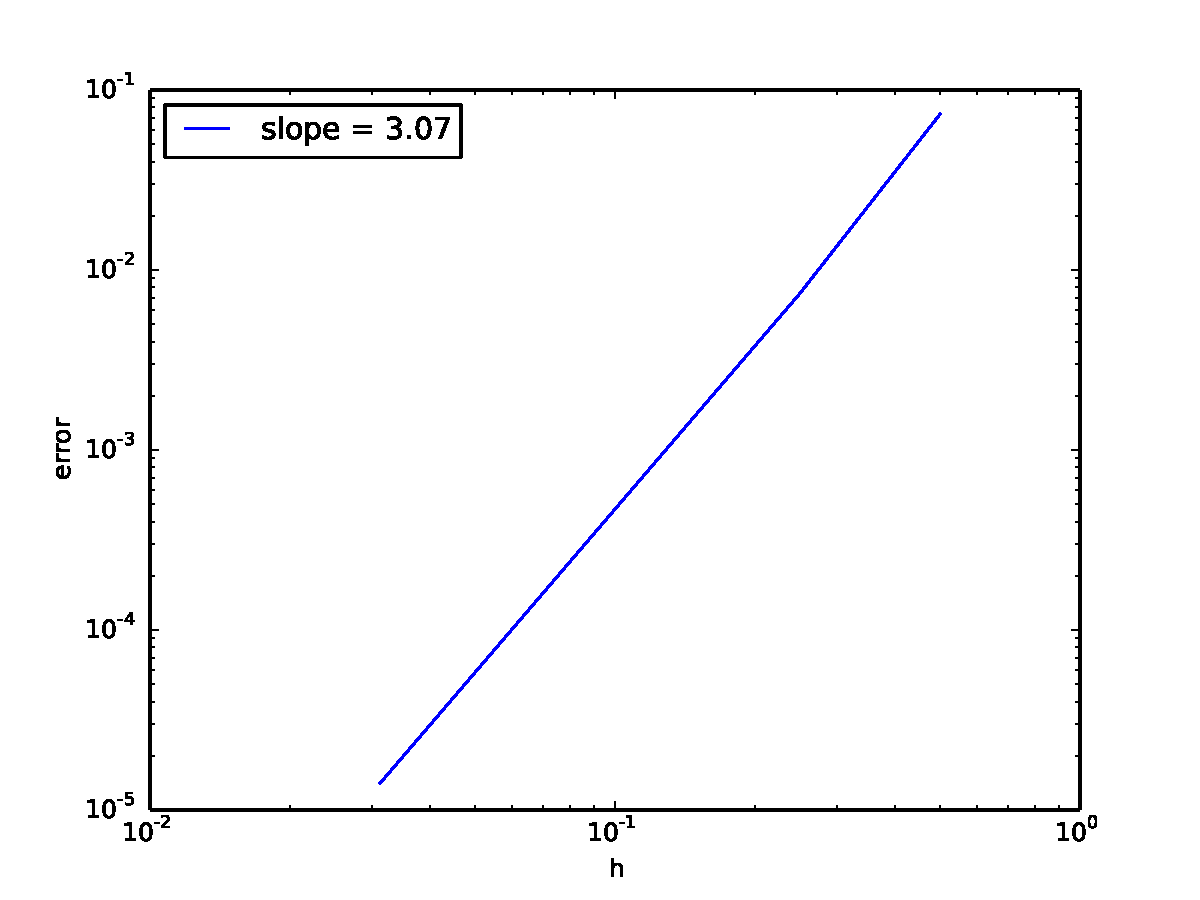
\includegraphics[width=0.7\textwidth]{SpaceTimeHeat/convergence}
	\caption{$L^2$ convergence of $u$ for the space-time heat equation}
	\label{fig:spaceTimeHeatConvergence}
\end{figure}

In order to demonstrate local space-time adaptivity we consider one more problem for the heat equation. 
On the same domain, and with the same boundary conditions as the previous example, we let the initial heat distribution be zero.
Then between $t=0.25$ and $t=0.5$ we turn on a pulse source term of one on $0.375\leq x\leq 0.625$. 
Starting from an initial mesh of $4x4$, we adaptively refine four times and obtain the results in Figure \ref{fig:spaceTimeHeatPulse}.
Notice that $\hat u$ in Figure \ref{fig:spaceTimeHeatuhat} only lives on vertical edges as was discussed earlier.
Also notice that the full mesh shown in Figure \ref{fig:spaceTimeHeatfhat} automatically adapts spatially and temporally to where features are rapidly changing. 

\begin{figure}[ht]
\centering
\begin{subfigure}[t]{0.45\textwidth}
\centering
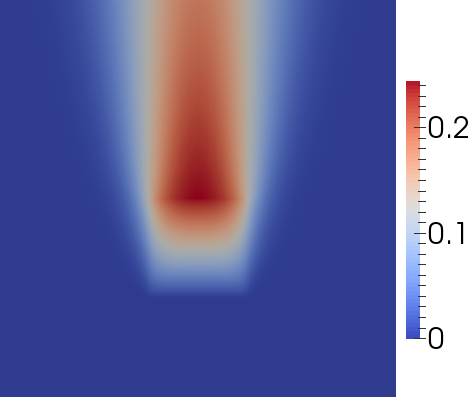
\includegraphics[width=\textwidth]{SpaceTimeHeat/PulseSource/u.png}
\caption{$u$}
\label{fig:spaceTimeHeatu}
\end{subfigure}
\begin{subfigure}[t]{0.45\textwidth}
\centering
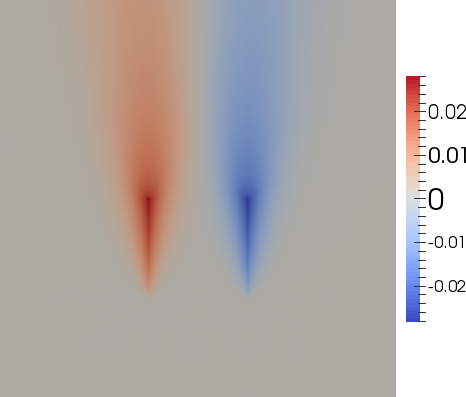
\includegraphics[width=\textwidth]{SpaceTimeHeat/PulseSource/sigma.png}
\caption{$\sigma$}
\label{fig:spaceTimeHeatsigma}
\end{subfigure}
\begin{subfigure}[t]{0.45\textwidth}
\centering
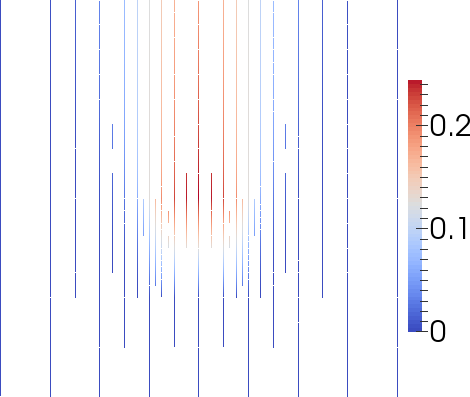
\includegraphics[width=\textwidth]{SpaceTimeHeat/PulseSource/uhat.png}
\caption{$\hat u$}
\label{fig:spaceTimeHeatuhat}
\end{subfigure}
\begin{subfigure}[t]{0.45\textwidth}
\centering
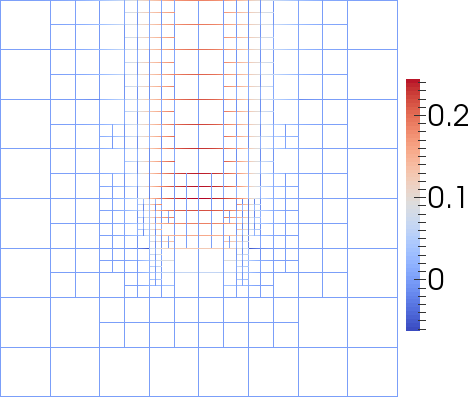
\includegraphics[width=\textwidth]{SpaceTimeHeat/PulseSource/fhat.png}
\caption{$\hat t$}
\label{fig:spaceTimeHeatfhat}
\end{subfigure}
\caption{Pulsed space-time heat problem after 4 refinements}
\label{fig:spaceTimeHeatPulse}
\end{figure}

%    /$$$$$$                                                                            /$$ /$$       /$$          
%   /$$__  $$                                                                          |__/| $$      | $$          
%  | $$  \__/  /$$$$$$  /$$$$$$/$$$$   /$$$$$$   /$$$$$$   /$$$$$$   /$$$$$$$  /$$$$$$$ /$$| $$$$$$$ | $$  /$$$$$$ 
%  | $$       /$$__  $$| $$_  $$_  $$ /$$__  $$ /$$__  $$ /$$__  $$ /$$_____/ /$$_____/| $$| $$__  $$| $$ /$$__  $$
%  | $$      | $$  \ $$| $$ \ $$ \ $$| $$  \ $$| $$  \__/| $$$$$$$$|  $$$$$$ |  $$$$$$ | $$| $$  \ $$| $$| $$$$$$$$
%  | $$    $$| $$  | $$| $$ | $$ | $$| $$  | $$| $$      | $$_____/ \____  $$ \____  $$| $$| $$  | $$| $$| $$_____/
%  |  $$$$$$/|  $$$$$$/| $$ | $$ | $$| $$$$$$$/| $$      |  $$$$$$$ /$$$$$$$/ /$$$$$$$/| $$| $$$$$$$/| $$|  $$$$$$$
%   \______/  \______/ |__/ |__/ |__/| $$____/ |__/       \_______/|_______/ |_______/ |__/|_______/ |__/ \_______/
%                                    | $$                                                                          
%                                    | $$                                                                          
%                                    |__/    
\section{Transient Compressible Navier-Stokes}
The compressible Navier-Stokes equations are
\begin{align}
\frac{\partial}{\partial t}\svectthree{\rho}{\rho\bfu}{\rho e_0}
+\Div\svectthree{\rho\bfu}{\rho\bfu\otimes\bfu+p\bfI-\mathbb{D}}{\rho\bfu e_0+\bfu p+\bfq-\bfu\cdot\mathbb{D}}
%TODO: Possible error above. cfd-online seems to have T^T
=\svectthree{f_c}{\bff_m}{f_e}\,,
\end{align}
where $\rho$ is the density, $\bfu$ is the velocity, $p$ is the pressure, $\bfI$ is the identity matrix,
$\mathbb{D}$ is the deviatoric stress tensor or viscous stress, $e_0$ is the total energy, $\bfq$ is the heat flux, 
and $f_c$, $\bff_m$, and $f_e$ are the source terms for the continuity, momentum, and energy equations, respectively.
Assuming Stokes hypothesis that $\lambda=-\frac{2}{3}\mu$, 
\begin{equation*}
	\mathbb{D}=2\mu\bfS^*=2\mu\LRs{\frac{1}{2}\LRp{\Grad\bfu+\LRp{\Grad\bfu}^T}-\frac{1}{3}\Div\bfu\bfI}\,,
\end{equation*}
where $\bfS^*$ is the trace-less viscous strain rate tensor.
The heat flux is given by Fourier's law:
\begin{equation*}
	\bfq=-C_p\frac{\mu}{Pr}\Grad T\,,
\end{equation*}
where $C_p$ is the specific heat at constant pressure and $Pr$ is the laminar Prandtl number: $Pr:=\frac{C_p\mu}{\lambda}$.
We need to close these equations with an equation of state. An ideal gas assumption gives
\begin{equation*}
	\gamma:=\frac{C_p}{C_v}\,,\quad p=\rho RT\,,\quad e=C_v T\,,\quad C_p-C_v=R\,,
\end{equation*}
where $\gamma$ is the ratio of specific heats, $C_v$ is the specific heat at constant volume, $R$ is the gas constant,
$e$ is the internal energy, $T$ is the temperature,
and $\gamma$, $C_p$, $C_v$, and $R$ are constant properties of the fluid.
The total energy is defined by
\begin{equation*}
	e_0=e+\frac{1}{2}\bfu\cdot\bfu\,.
\end{equation*}

We can write our first order system of equations in space-time as follows:
\begin{subequations}
\label{eq:compressibleNSFirstOrder}
\begin{align}
	\frac{1}{\mu}\mathbb{D}-\LRp{\Grad\bfu+\LRp{\Grad\bfu}^T}+\frac{2}{3}\Div\bfu\bfI&=0\\
	\frac{Pr}{C_p\mu}\bfq+\Grad T&=0\\
	\Divxt\vecttwo{\rho\bfu}{\rho}&=f_c\\
	\Divxt\vecttwo{\rho\bfu\otimes\bfu+\rho RT\bfI-\mathbb{D}}{\rho\bfu}&=\bff_m\\
	\Divxt\vecttwo{\rho\bfu\LRp{C_v T+\frac{1}{2}\bfu\cdot\bfu}+\bfu\rho RT+\bfq-\bfu\cdot\mathbb{D}}{\rho\LRp{C_v T+\frac{1}{2}\bfu\cdot\bfu}}&=f_e\,,
\end{align}
\end{subequations}
where our solution variables are $\rho$, $\bfu$, $T$, $\mathbb{D}$, and $\bfq$.

%   /$$$$$$$                      /$$                        /$$     /$$                    
%  | $$__  $$                    |__/                       | $$    |__/                    
%  | $$  \ $$  /$$$$$$   /$$$$$$  /$$ /$$    /$$  /$$$$$$  /$$$$$$   /$$  /$$$$$$  /$$$$$$$ 
%  | $$  | $$ /$$__  $$ /$$__  $$| $$|  $$  /$$/ |____  $$|_  $$_/  | $$ /$$__  $$| $$__  $$
%  | $$  | $$| $$$$$$$$| $$  \__/| $$ \  $$/$$/   /$$$$$$$  | $$    | $$| $$  \ $$| $$  \ $$
%  | $$  | $$| $$_____/| $$      | $$  \  $$$/   /$$__  $$  | $$ /$$| $$| $$  | $$| $$  | $$
%  | $$$$$$$/|  $$$$$$$| $$      | $$   \  $/   |  $$$$$$$  |  $$$$/| $$|  $$$$$$/| $$  | $$
%  |_______/  \_______/|__/      |__/    \_/     \_______/   \___/  |__/ \______/ |__/  |__/
%                                                                                           
%                                                                                           
%              
\subsection{Derivation of Space-Time DPG Formulation}
We start with \eqref{eq:compressibleNSFirstOrder} and multiply by test functions $\mathbb{S}$ (symmetric tensor), $\bftau$, $v_c$, $\bfv_m$, $v_e$, 
then integrate by parts over each space-time element $K$:
\begin{subequations}
\label{eq:compressibleNSBF}
\begin{align}
	\LRp{\frac{1}{\mu}\mathbb{D},\mathbb{S}}+\LRp{2\bfu,\Div\mathbb{S}}-\LRp{\frac{2}{3}\bfu,\Grad\trace{\mathbb{S}}}
	-\LRa{\frac{4}{3}\hat\bfu,\mathbb{S}\bfn_x}&=0\\
	\LRp{\frac{Pr}{C_p\mu}\bfq,\bftau}-\LRp{T,\Div\bftau}+\LRa{\hat T,\tau_n}&=0\\
	-\LRp{\vecttwo{\rho\bfu}{\rho},\Gradxt v_c}+\LRa{\hat t_c,v_c}&=\LRp{f_c,v_c}\\
	-\LRp{\vecttwo{\rho\bfu\otimes\bfu+\rho RT\bfI-\mathbb{D}}{\rho\bfu},\Gradxt\bfv_m}+\LRa{\hat\bft_m,\bfv_m}&=\LRp{\bff_m,\bfv_m}\\
	-\LRp{\vecttwo{\rho\bfu\LRp{C_v T+\frac{1}{2}\bfu\cdot\bfu}+\bfu\rho RT+\bfq-\bfu\cdot\mathbb{D}}{\rho\LRp{C_v T+\frac{1}{2}\bfu\cdot\bfu}},\Gradxt v_e}
	+\LRa{\hat t_e,v_e}&=\LRp{f_e,v_e}\,,
\end{align}
\end{subequations}
where 
\begin{equation*}
\begin{aligned}
\hat\bfu&=\trace(\bfu)\\
\hat T&=\trace(T)\\
\hat t_c&=\trace\LRp{\rho\bfu}\cdot\bfn_x
+\trace\LRp{\rho}n_t\\
\hat\bft_m&=\trace\LRp{\rho\bfu\otimes\bfu+\rho RT\bfI-\mathbb{D}}\cdot\bfn_x
+\trace\LRp{\rho\bfu} n_t\\
\hat t_e&=\trace\LRp{\rho\bfu\LRp{C_v T+\frac{1}{2}\bfu\cdot\bfu}+\bfu\rho RT+\bfq-\bfu\cdot\mathbb{D}}\cdot\bfn_x
+\trace\LRp{\rho\LRp{C_v T+\frac{1}{2}\bfu\cdot\bfu}}n_t\,.
\end{aligned}
\end{equation*}
Note that integrating $\mathbb{S}$ against the symmetric gradient only picks up the symmetric part.
This is a much more complicated system of equations than we had for the space-time heat equation, but the situation has many similarities.
Test function $\bftau\in\HdivK$ where the divergence is taken only over spatial dimensions, $v_c,v_e\in\HOneK$, and $\bfv_m\in\HOneVecK$.
These are all familiar spaces from our work with the heat equation.
Unfortunately, $\mathbb{S}$ has some weird requirements: each $d\times d$ components must be at least in $L^2(K)$, $\Div\mathbb{S}\in\LVecK$, and
$\Grad\trace{\mathbb{S}}\in\LVecK$.
In practice, we will probably just seek each component in $\HOneK$.

%   /$$       /$$                                         /$$                       /$$     /$$                    
%  | $$      |__/                                        |__/                      | $$    |__/                    
%  | $$       /$$ /$$$$$$$   /$$$$$$   /$$$$$$   /$$$$$$  /$$ /$$$$$$$$  /$$$$$$  /$$$$$$   /$$  /$$$$$$  /$$$$$$$ 
%  | $$      | $$| $$__  $$ /$$__  $$ |____  $$ /$$__  $$| $$|____ /$$/ |____  $$|_  $$_/  | $$ /$$__  $$| $$__  $$
%  | $$      | $$| $$  \ $$| $$$$$$$$  /$$$$$$$| $$  \__/| $$   /$$$$/   /$$$$$$$  | $$    | $$| $$  \ $$| $$  \ $$
%  | $$      | $$| $$  | $$| $$_____/ /$$__  $$| $$      | $$  /$$__/   /$$__  $$  | $$ /$$| $$| $$  | $$| $$  | $$
%  | $$$$$$$$| $$| $$  | $$|  $$$$$$$|  $$$$$$$| $$      | $$ /$$$$$$$$|  $$$$$$$  |  $$$$/| $$|  $$$$$$/| $$  | $$
%  |________/|__/|__/  |__/ \_______/ \_______/|__/      |__/|________/ \_______/   \___/  |__/ \______/ |__/  |__/
%                                                                                                                  
%                                                                                                                  
%   
\subsubsection{Linearization}
We follow a standard residual-Jacobian linearization procedure coupled with a Gauss-Newton solve.
Let $U=\LRc{\rho,\bfu,T,\mathbb{D},\bfq,\hat\bfu,\hat e,\hat t_c,\hat\bft_m,\hat t_e}$ be a group solution variable which we can decompose into two parts:
$U:=\tilde U+\Delta U$, where
$\tilde U = \LRc{\tilde\rho,\tilde\bfu,\tilde T,\tilde{\mathbb{D}},\bs0,\bs0,0,0,\bs0,0}$ is the previous iteration approximation, 
and $\Delta U=\LRc{\Delta\rho,\Delta\bfu,\Delta T,\Delta\mathbb{D},\bfq,\hat\bfu,\hat e,\hat t_c,\hat\bft_m,\hat t_e}$ is the update.
Note that $\tilde U$ only contains terms which participate in nonlinearities in \eqref{eq:compressibleNSBF} 
while $\Delta U$ contains the full linear terms and the updates to the nonlinear terms.
Also, we drop the $\Delta$ and $\tilde\cdot$ notation for linear terms.
Define residual $R(U)$ as the left hand side of \eqref{eq:compressibleNSBF} minus the right hand side.
% Let $\tilde U$ be an approximate solution for the minimization of the residual. 
% We wish to solve for an increment $\Delta U$ such that $U=\tilde U+\Delta U$ is a better approximation of the true solution.
Approximating $R(U)=0$ by $R(\tilde U)+R'(\tilde U)\Delta U=0$, where $R'(\tilde U)$ is the Jacobian of $R$ evaluated at $\tilde U$, we get a linear system:
\begin{equation}
	R'(\tilde U)\Delta U=-R(\tilde U)\,.
\end{equation}
We only need to define our Jacobian and residual for each component of \eqref{eq:compressibleNSBF}. 
% Note that we can exclude our traces and fluxes from the residual since these unknowns are only involved in linear terms.
% As such, we don't update these variables each iteration based on the previous iteration.
% Instead, for example, we consider $\tilde{\hat\bfu}=0$, and let $\hat\bfu=\Delta\hat\bfu$ after each iteration.
% To indicate this different treatment, we drop the delta and tilde notation on these variables in the following discussion.
The Jacobian of our compressible Navier-Stokes system, $R'(\tilde U)\Delta U$ is
\begin{equation}
\label{eq:compressibleJacobian}
\begin{aligned}
	&\LRp{\frac{1}{\mu}\Delta\mathbb{D},\mathbb{S}}+\LRp{2\Delta\bfu,\Div\mathbb{S}}-\LRp{\frac{2}{3}\Delta\bfu,\Grad\trace{\mathbb{S}}}
	-\LRa{\frac{4}{3}\hat\bfu,\mathbb{S}\bfn_x}\\
	%
	&+\LRp{\frac{Pr}{C_p\mu}\bfq,\bftau}-\LRp{\Delta T,\Div\bftau}+\LRa{\hat T,\tau_n}\\
	%
	&-\LRp{\vecttwo{\Delta\rho\tilde\bfu+\tilde\rho\Delta\bfu}
	{\Delta\rho},\Gradxt v_c}
	+\LRa{\hat t_c,v_c}\\
	%
	&-\LRp{\vecttwo{\Delta\rho\tilde\bfu\otimes\tilde\bfu+\tilde\rho\Delta\bfu\otimes\tilde\bfu+\tilde\rho\tilde\bfu\otimes\Delta\bfu
	+\LRp{\Delta\rho R\tilde T+\tilde\rho R\Delta T}\bfI-\Delta\mathbb{D}}
	{\Delta\rho\tilde\bfu+\tilde\rho\Delta\bfu},\Gradxt\bfv_m}
	+\LRa{\hat\bft_m,\bfv_m}\\
	%
	&-\LRp{\vectthree{[C_v\Delta\rho\tilde T\tilde\bfu+C_v\tilde\rho\Delta T\tilde\bfu+C_v\tilde\rho\tilde T\Delta\bfu
	+\frac{1}{2}\LRp{\Delta\rho\tilde\bfu\cdot\tilde\bfu\tilde\bfu+\tilde\rho\Delta\bfu\cdot\tilde\bfu\tilde\bfu
	+\tilde\rho\tilde\bfu\cdot\Delta\bfu\tilde\bfu+\tilde\rho\tilde\bfu\cdot\tilde\bfu\Delta\bfu}}
	{+R\LRp{\Delta\rho\tilde T\tilde\bfu+\tilde\rho\Delta T\tilde\bfu+\tilde\rho\tilde T\Delta\bfu}
	+\bfq-\Delta\bfu\cdot\tilde{\mathbb{D}}-\tilde\bfu\cdot\Delta\mathbb{D}]}
	{C_v\Delta\rho\tilde T+C_v\tilde\rho\Delta T
	+\frac{1}{2}\LRp{\Delta\rho\tilde\bfu\cdot\tilde\bfu+\tilde\rho\Delta\bfu\cdot\tilde\bfu+\tilde\rho\tilde\bfu\cdot\Delta\bfu}},\Gradxt v_e}\\
	&+\LRa{\hat t_e,v_e}\,.
\end{aligned}
\end{equation}
The residual, $R(\tilde U)$, is then
\begin{equation}
\begin{aligned}
	&\LRp{\frac{1}{\mu}\tilde{\mathbb{D}},\mathbb{S}}+\LRp{2\tilde\bfu,\Div\mathbb{S}}-\LRp{\frac{2}{3}\tilde\bfu,\Grad\trace{\mathbb{S}}}\\
	&-\LRp{\tilde T,\Div\bftau}\\
	&-\LRp{\vecttwo{\tilde\rho\tilde\bfu}{\tilde\rho},\Gradxt v_c}-\LRp{f_c,v_c}\\
	&-\LRp{\vecttwo{\tilde\rho\tilde\bfu\otimes\tilde\bfu+\tilde\rho R\tilde T\bfI-\tilde{\mathbb{D}}}{\tilde\rho\tilde\bfu},
	\Gradxt\bfv_m}-\LRp{\bff_m,\bfv_m}\\
	&-\LRp{\vecttwo{\tilde\rho\tilde\bfu\LRp{C_v\tilde T+\frac{1}{2}\tilde\bfu\cdot\tilde\bfu}+\tilde\bfu\tilde\rho R\tilde T
	-\tilde\bfu\cdot\tilde{\mathbb{D}}}{\tilde\rho\LRp{C_v\tilde T+\frac{1}{2}\tilde\bfu\cdot\tilde\bfu}},
	\Gradxt v_e}-\LRp{f_e,v_e}\,.
\end{aligned}
\end{equation}

%   /$$$$$$$$                       /$$           /$$   /$$                                  
%  |__  $$__/                      | $$          | $$$ | $$                                  
%     | $$     /$$$$$$   /$$$$$$$ /$$$$$$        | $$$$| $$  /$$$$$$   /$$$$$$  /$$$$$$/$$$$ 
%     | $$    /$$__  $$ /$$_____/|_  $$_/        | $$ $$ $$ /$$__  $$ /$$__  $$| $$_  $$_  $$
%     | $$   | $$$$$$$$|  $$$$$$   | $$          | $$  $$$$| $$  \ $$| $$  \__/| $$ \ $$ \ $$
%     | $$   | $$_____/ \____  $$  | $$ /$$      | $$\  $$$| $$  | $$| $$      | $$ | $$ | $$
%     | $$   |  $$$$$$$ /$$$$$$$/  |  $$$$/      | $$ \  $$|  $$$$$$/| $$      | $$ | $$ | $$
%     |__/    \_______/|_______/    \___/        |__/  \__/ \______/ |__/      |__/ |__/ |__/
%                                                                                            
%                                                                                            
%      
\subsubsection{Test Norm}
The most obvious first choice for test norm in the local solve is the graph norm, which comes from the 
problem adjoint.
We start by grouping terms in \eqref{eq:compressibleJacobian} by trial variable to get
\begin{equation}
\begin{aligned}
&\LRp{\Delta\mathbb{D},\frac{1}{\mu}\mathbb{S}+\Grad\bfv_m+\Grad v_e\otimes\tilde\bfu}\\
+&\LRp{\bfq,\frac{Pr}{C_p\mu}\bftau-\Grad v_e}\\
+&\left(\Delta\rho,-\tilde\bfu\cdot\Grad v_c-\frac{\partial v_c}{\partial t}
-\tilde\bfu\otimes\tilde\bfu:\Grad\bfv_m
-R\tilde T\Div\bfv_m-\tilde\bfu\cdot\frac{\partial\bfv_m}{\partial t}\right.\\
&\left.-C_v\tilde T\tilde\bfu\cdot\Grad v_e-\frac{1}{2}\tilde\bfu\cdot\tilde\bfu\tilde\bfu\cdot\Grad v_e
-R\tilde T\tilde\bfu\Grad v_e
-C_v\tilde T\frac{\partial v_e}{\partial t}-\frac{1}{2}\tilde\bfu\cdot\tilde\bfu\frac{\partial v_e}{\partial t}
\right)\\
+&\left(\Delta\bfu,2\Div\mathbb{S}-\frac{2}{3}\Grad\trace{\mathbb{S}}
-\tilde\rho\Grad v_c
-\tilde\rho\tilde\bfu\cdot\Grad\bfv_m-\tilde\rho\Grad\bfv_m\cdot\tilde\bfu
-\tilde\rho\frac{\partial\bfv_m}{\partial t}
-C_v\tilde\rho\tilde T\Grad v_e\right.\\
&\left.
-\frac{1}{2}\tilde\rho\tilde\bfu\cdot\tilde\bfu\Grad v_e
-\frac{1}{2}\tilde\rho\tilde\bfu\cdot\Grad v_e\tilde\bfu
-\frac{1}{2}\tilde\rho\Grad v_e\cdot\tilde\bfu\tilde\bfu
-R\tilde\rho\tilde T_\Grad v_e
+\tilde{\mathbb{D}}\cdot\Grad v_e
-\frac{1}{2}\tilde\rho\tilde\bfu\frac{\partial v_e}{\partial t}
-\frac{1}{2}\tilde\rho\tilde\bfu\frac{\partial v_e}{\partial t}
\right)\\
+&\left(\Delta T,-\Div\bftau
-R\tilde\rho\Div\bfv_m
-C_v\tilde\rho\tilde\bfu\Grad v_e
-R\tilde\rho\tilde\bfu\Grad v_e
-C_v\tilde\rho\frac{\partial v_e}{\partial t}
\right)\\
+&\LRp{\hat\bfu,-\frac{4}{3}\mathbb{S}\bfn_x}\\
+&\LRp{\hat T,\tau_n}\\
+&\LRp{\hat t_c,v_c}\\
+&\LRp{\hat\bft_m,\bfv_m}\\
+&\LRp{\hat t_e,v_e}\,.
\end{aligned}	
\end{equation}

Then the graph norm would be defined by
\begin{equation}
\begin{aligned}
&\norm{\frac{1}{\mu}\mathbb{S}+\Grad\bfv_m+\Grad v_e\otimes\tilde\bfu}^2\\
+&\norm{\frac{Pr}{C_p\mu}\bftau-\Grad v_e}^2\\
+&\left\|
-\tilde\bfu\cdot\Grad v_c-\frac{\partial v_c}{\partial t}-\tilde\bfu\otimes\tilde\bfu:\Grad\bfv_m
-R\tilde T\Div\bfv_m-\tilde\bfu\cdot\frac{\partial\bfv_m}{\partial t}\right.\\
&\left.-C_v\tilde T\tilde\bfu\cdot\Grad v_e-\frac{1}{2}\tilde\bfu\cdot\tilde\bfu\tilde\bfu\cdot\Grad v_e
-R\tilde T\tilde\bfu\Grad v_e
-C_v\tilde T\frac{\partial v_e}{\partial t}-\frac{1}{2}\tilde\bfu\cdot\tilde\bfu\frac{\partial v_e}{\partial t}
\right\|^2\\
+&\left\|2\Div\mathbb{S}-\frac{2}{3}\Grad\trace{\mathbb{S}}
-\tilde\rho\Grad v_c
-\tilde\rho\tilde\bfu\cdot\Grad\bfv_m-\tilde\rho\Grad\bfv_m\cdot\tilde\bfu
-\tilde\rho\frac{\partial\bfv_m}{\partial t}
-C_v\tilde\rho\tilde T\Grad v_e\right.\\
&\left.
-\frac{1}{2}\tilde\rho\tilde\bfu\cdot\tilde\bfu\Grad v_e
-\frac{1}{2}\tilde\rho\tilde\bfu\cdot\Grad v_e\tilde\bfu
-\frac{1}{2}\tilde\rho\Grad v_e\cdot\tilde\bfu\tilde\bfu
-R\tilde\rho\tilde T\Grad v_e
+\tilde{\mathbb{D}}\cdot\Grad v_e
-\frac{1}{2}\tilde\rho\tilde\bfu\frac{\partial v_e}{\partial t}
-\frac{1}{2}\tilde\rho\tilde\bfu\frac{\partial v_e}{\partial t}
\right\|^2\\
+&\left\|-\Div\bftau
-R\tilde\rho\Div\bfv_m
-C_v\tilde\rho\tilde\bfu\Grad v_e
-R\tilde\rho\tilde\bfu\Grad v_e
-C_v\tilde\rho\frac{\partial v_e}{\partial t}
\right\|\\
+&\alpha_c\norm{v_c}^2
+\alpha_m\norm{\bfv_m}^2
+\alpha_e\norm{v_e}^2
\,,
\end{aligned}
\end{equation}
where $\alpha_c$, $\alpha_m$, and $\alpha_e$ are scaling constants.

%   /$$$$$$$$             /$$                                  
%  | $$_____/            | $$                                  
%  | $$       /$$   /$$ /$$$$$$   /$$   /$$  /$$$$$$   /$$$$$$ 
%  | $$$$$   | $$  | $$|_  $$_/  | $$  | $$ /$$__  $$ /$$__  $$
%  | $$__/   | $$  | $$  | $$    | $$  | $$| $$  \__/| $$$$$$$$
%  | $$      | $$  | $$  | $$ /$$| $$  | $$| $$      | $$_____/
%  | $$      |  $$$$$$/  |  $$$$/|  $$$$$$/| $$      |  $$$$$$$
%  |__/       \______/    \___/   \______/ |__/       \_______/
%                                                              
%                                                              
%  
\section{Challenges and Future Work}

\subsection{Preconditioning and Iterative Solvers}

%    /$$$$$$                                /$$                     /$$                              
%   /$$__  $$                              | $$                    |__/                              
%  | $$  \__/  /$$$$$$  /$$$$$$$   /$$$$$$$| $$ /$$   /$$  /$$$$$$$ /$$  /$$$$$$  /$$$$$$$   /$$$$$$$
%  | $$       /$$__  $$| $$__  $$ /$$_____/| $$| $$  | $$ /$$_____/| $$ /$$__  $$| $$__  $$ /$$_____/
%  | $$      | $$  \ $$| $$  \ $$| $$      | $$| $$  | $$|  $$$$$$ | $$| $$  \ $$| $$  \ $$|  $$$$$$ 
%  | $$    $$| $$  | $$| $$  | $$| $$      | $$| $$  | $$ \____  $$| $$| $$  | $$| $$  | $$ \____  $$
%  |  $$$$$$/|  $$$$$$/| $$  | $$|  $$$$$$$| $$|  $$$$$$/ /$$$$$$$/| $$|  $$$$$$/| $$  | $$ /$$$$$$$/
%   \______/  \______/ |__/  |__/ \_______/|__/ \______/ |_______/ |__/ \______/ |__/  |__/|_______/ 
%                                                                                                    
%                                                                                                    
%
\section{Conclusions}

\bibliographystyle{plain}
\bibliography{../LCPaper}
\end{document}

